\documentclass{beamer}

% El color y el tema de la presentación
\usetheme{madrid}
\usecolortheme{seahorse}

\setbeamertemplate{navigation symbols}{}
\setbeamercovered{transparent}
\usepackage[utf8]{inputenc}
\usepackage[T1]{fontenc}

\usepackage{Sweave}
\begin{document}
\Sconcordance{concordance:presentacion_Parada_G_M8R2.tex:presentacion_Parada_G_M8R2.Rnw:1 %
11 1 1 0 37 1 1 29 19 0 1 2 20 1 1 25 1 4 17 1 1 12 1 3 19 1 1 11 1 3 %
27 1}



\begin{frame}
\frametitle{Esperanza de Vida y GDP PPP en Suramérica (1875-2025)}
\framesubtitle{Autor: Gabriel Parada}
Agosto 2025

\end{frame}


\begin{frame}
\frametitle{Introducción}

\begin{itemize}
\item<1-> El presente trabajo investiga el nivel de la \textbf{Esperanza de Vida} desde el año 1875 hasta el 2025 en Suramérica y su relación con el \textbf{GDP per cápita (PPP)}. 
\item<2-> Se usan dos datasets de Gapminder.
\end{itemize}

\end{frame}

\begin{frame}
\frametitle{Introducción}

\begin{itemize}
\item<1> \textbf{Esperanza de Vida:} La esperanza de vida es el número promedio de años que se espera que viva una persona desde su nacimiento, considerando las condiciones de mortalidad de un período específico.

\item<2> \textbf{GDP per cápita PPP:} Es una medida de la producción económica per cápita de un país, ajustada por las diferencias en el costo de vida y los tipos de cambio entre países.	
\end{itemize}


\end{frame}

\begin{frame}[fragile]
\frametitle{Estadísticas Descriptivas 1875-2025}

{\scriptsize
% latex table generated in R 4.4.0 by xtable 1.8-4 package
% Sat Aug  9 21:27:56 2025
\begin{table}[ht]
\centering
\begin{tabular}{lrrrrrr}
  \hline
Países & min.E.Vida & max.E.Vida & diff.E.Vida & min.GDP & max.GDP & diff.GDP \\ 
  \hline
Argentina & 32.91 & 77.60 & 44.69 & 2910 & 24600 & 21690 \\ 
  Bolivia & 27.21 & 73.47 & 46.26 & 1490 & 8530 & 7040 \\ 
  Brazil & 25.97 & 77.09 & 51.12 & 973 & 16000 & 15027 \\ 
  Chile & 26.85 & 81.39 & 54.54 & 2180 & 26700 & 24520 \\ 
  Colombia & 30.26 & 81.37 & 51.11 & 1220 & 15900 & 14680 \\ 
  Ecuador & 30.13 & 77.51 & 47.38 & 870 & 11300 & 10430 \\ 
  Guyana & 27.43 & 68.26 & 40.83 & 2020 & 72800 & 70780 \\ 
  Peru & 28.79 & 81.49 & 52.70 & 870 & 13000 & 12130 \\ 
  Uruguay & 30.36 & 78.50 & 48.14 & 3540 & 25900 & 22360 \\ 
  Venezuela & 30.73 & 76.18 & 45.45 & 1830 & 21000 & 19170 \\ 
   \hline
\end{tabular}
\end{table}}
\end{frame}

\begin{frame}[fragile]
\frametitle{Estadísticas Descriptivas 1875-2025}

\begin{itemize}
\item<1> Los 10 países del estudio han aumentado su esperanza de vida en promedio 
48 años en los últimos 
150 años.

\item<2> Los 10 países del estudio han aumentado su GDP promedio en 
21.783 \$
dólares en un periodo de 150 años.

\end{itemize}
\end{frame}

\begin{frame}{fragile}
\frametitle{Histograma Esperanza de vida en Suramérica (1875 - 2025)}

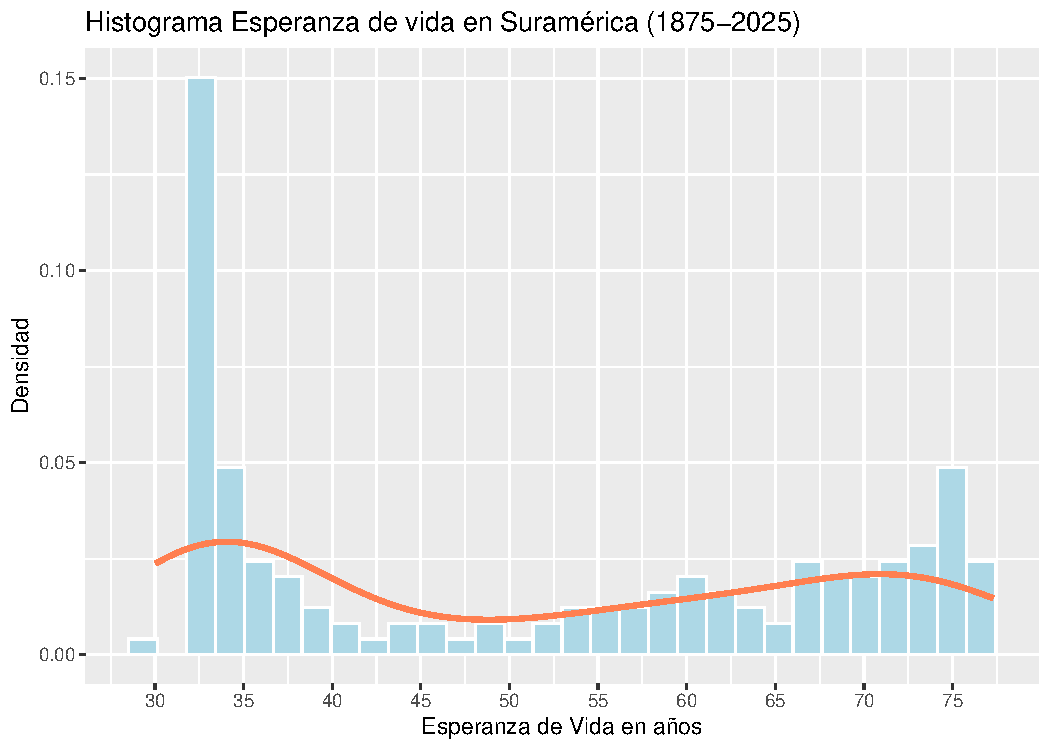
\includegraphics{presentacion_Parada_G_M8R2-002}

\end{frame}

\begin{frame}[fragile]
\frametitle{Estadísticas Descriptivas 1875–2025}

\begin{itemize}
\item<1> Al observar la distribución de densidad de la Esperanza de Vida de los países de Suramérica en los últimos 150 años se nota que un tercio de la misma se situa entre los 30 y 37.5 años.

\item<2> Luego incrementa rápidamente y se estabiliza un poco entre el rango de 70 a 80 años.

\end{itemize}
\end{frame}


\begin{frame}{fragile}
\frametitle{Esperanza de vida por país}

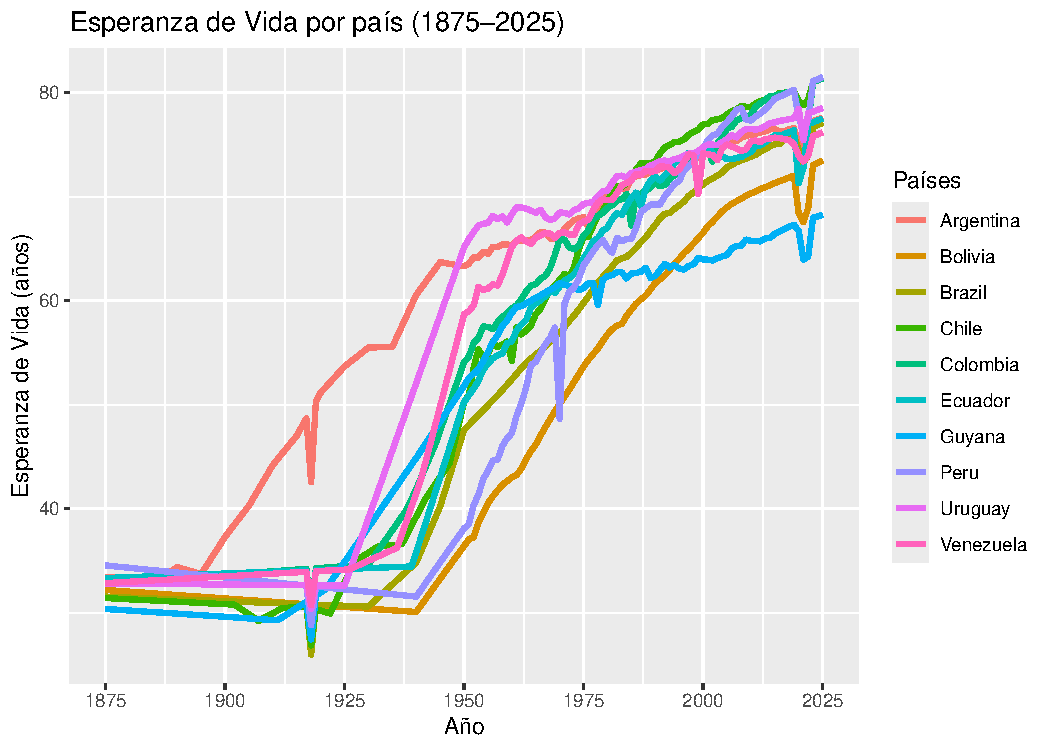
\includegraphics{presentacion_Parada_G_M8R2-003}

\end{frame}

\begin{frame}[fragile]
\frametitle{Esperanza de vida por país}

\begin{itemize}
\item<1> Entre 1925 y 1935 se observa un rápido incremento en la Esperanza de Vida.

\item<2> Bolivia y Guyana se han quedado rezagados en el aumento de la Esperanza de Vida. Guyana es uncaso interesante porque en los últimos años ha tenido un crecimiento económico acelerado, pero esto no se ha reflejado por los momentos en una mejora de la Esperanza de Vida.

\item<3> Argentina es un outlier gozando de un incremento de la Esperanza de Vida desde 1890. Algunas de las razones fueron: Un crecimiento económico temprano, urbanización controlada y políticas de salud pública pioneras hicieron que cayera de forma drástica la mortalidad infantil.

\end{itemize}
\end{frame}


\begin{frame}{fragile}
\frametitle{GDP per cápita PPP por país}

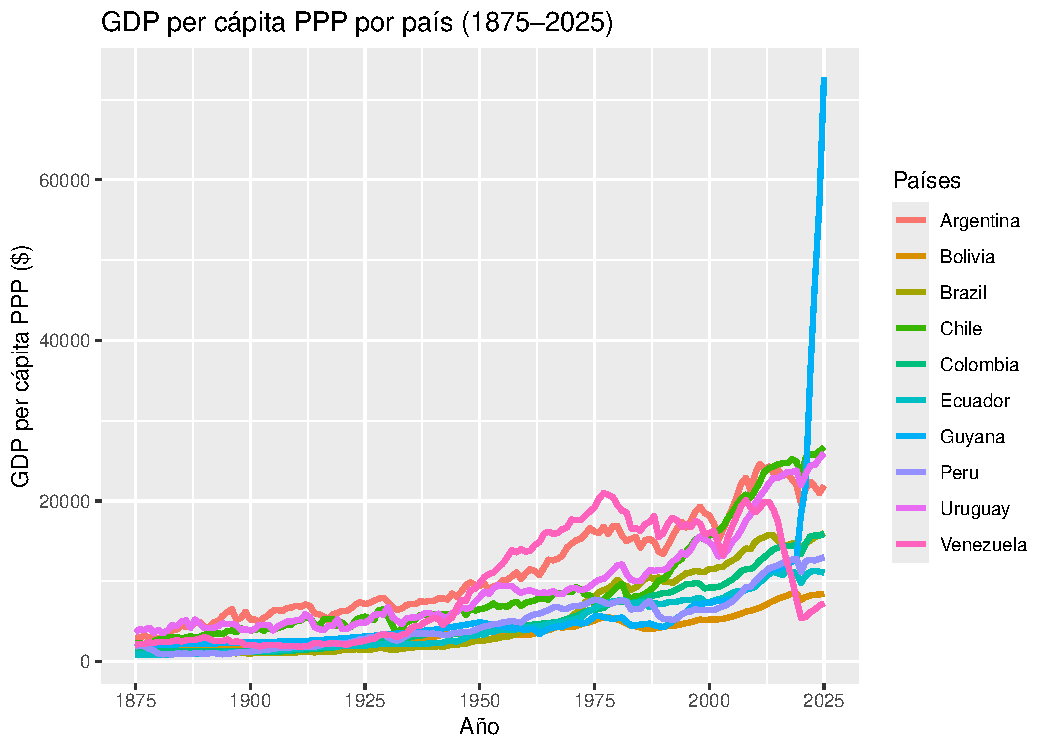
\includegraphics{presentacion_Parada_G_M8R2-004}

\end{frame}

\begin{frame}[fragile]
\frametitle{GDP per cápita PPP por país}

\begin{itemize}
\item<1> La tendencia general es que todos los países de Suramérica han aumentado su GDP per cápita PPP.

\item<2> Venezuela en terminos de GDP per cápita PPP fué entre los años 1950 y finales de la década de 1990 el país con mayor poder adquisitivo. Seguido por una grave crisis económica a inicios de la década del 2010.

\item<3> Guyana ha sido históricamente un país con un bajo GDP Per cápita PPP, pero en 2015 se descubrieron grandes pozos petroleros en sus costas. En el año 2019 empezó la explotación lo que ha aumentado su GDP per cápita PPP de 12800\$ en ese año hasta 72800\$ en el 2025 y se espera que continue este crecimiento económico.


\end{itemize}
\end{frame}











\end{document}
